\chapter{Построение математической модели}
\section{Постановка задачи}
Цель работы:
\begin{itemize}
	\item Сформулировать  модель двуиерного переноса.
	\item Выбрать схемы решения.
	\item Провести численные эксперименты с различными методами аппроксимайции, для понимания их влияния на решение.
	\item Провести анализ решений.
\end{itemize}

Дано:
\begin{itemize}

	\item ${(x,y)}$ - координаты  пространства,
	\item $t$ - время,
		\item  $u(x, y,t)$ - функция, задающая концентрацию вещества в любой момент времени (удельная масса или
		энергия (отнесенная к единице объема). 
		\item  $u(x,y,0)$ - поле переноса
	\item $\vec{v} = (v_{x}, v_{y}) $ - скорость переноса (\textit{const}),
	\item $f(x,y,t)$ - описывает источники и стоки,
\end{itemize}
\section{Формализация}
Будем рассматривать задачу для линейного уравнения переноса.
Для аппроксимации будем использовать два метода: неявная схема и метод Лагранжевых частиц.

\newpage
\section{Построение модели}
Рассмотрим газовую или жидкую сплошную среду. Примем: все точки среды
находятся в неравновесном состоянии. Это приводит к возникновению полей
концентраций, температур, давлений, а наличие градиентов этих параметров вызывает
перенос массы и энергии.

Выделим элемент объема движущейся жидкости в неоднородном поле некоторого
потенциала переноса. Под потенциалом переноса
$u$ понимают удельную массу или
энергию (отнесенную к единице объема).
$u (x, y, z, t)$ - скалярная величина.

Известно, что скалярная функция $u$  называется потенциалом вектороной функции $\vec{q}$, если между ними существует связь вида \cite{Alonso1992}:
\[
	\vec{q} = - \nabla u.
\]
Далее будем рассматривать связь, как пропорциональность.

Таким образом, поток переносимой субстанции (массы или энергии) является
векторной величиной $\vec{q}$.
В случае переноса массы под потенциалом переноса
$u$ обычно понимают
концентрацию компонента в смеси.

В рассматриваемой среде могут существовать, так называемые, объемные
(непрерывно распределенные по объему) источники или стоки массы и энергии. 
В химической технологии под ними подразумеваются химические превращения.

Известно, что процессы тепло- и массообмена осуществляются двумя основными
механизмами: молекулярным и конвективным. Молекулярный перенос (диффузия,
теплопроводность) возникает в результате стремления системы к термодинамическому
равновесию, а конвективный вызывается наличием поля скоростей в жидком или газовом
объеме V.

Следует отметить, что в случае переноса энергии в форме теплоты существует ещѐ
и радиантный перенос (тепловое излучение), вклад которого учитывают при достаточно
высоких температурах.

Процессы молекулярного переноса массы и энергии описываются
соответствующими феноменологическими уравнениями, являющимися, как правило,
линейными градиентными законами.

Опуская доказательство, изложенное в  \cite{Alonso1992}, можно сделать вывод:
в случае молекулярного и конвективного переноса общая
плотность потока массы или энергии складывается из двух векторных величин:
\[ \vec{q} = \vec{q}_{M} + \vec{q}_{K},\]
где $ \vec{q}_{M} $ - векторная величина молекулярного переноса, $ \vec{q}_{K} $ - векторная величина конвективного переноса.

В газовой или жидкой среде, находящейся в движении, выделим произвольный
объем $V$, ограниченный поверхностью $A$.
\begin{figure}[h]  % Окружение для картинки
	\centering
	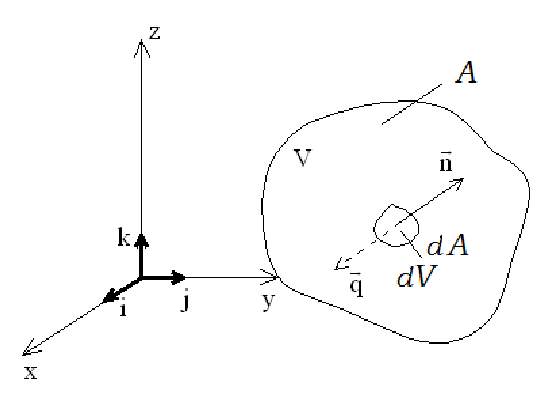
\includegraphics[height=0.5\textwidth]{imgs/area.png}  % Вставка изображения
	\caption{Объём серды, ограниченный поверхностью $A$}  % Подпись к изображению
	\label{fig:area}  % Метка для ссылки
\end{figure}
На поверхности $A$ выделим элемент
поверхности $dА$ и представим его в векторной форме, умножив на единичный вектор $\vec{n}$,
нормальный к этому элементу и направленный из объема, $\vec{n} dA = d\vec{A}$.

Составим балансовое уравнение:

\textbf{Накопление внутри объёма = вход - выход + образование.}

Примем, что в произвольном объеме нет источников субстанции или стоков, т.е.
образование равно нулю.

Плотность потока субстанции через площадку $d\vec{A}$ будет $-\vec{q}d\vec{A}$.
Знак минут интвертирует потоки (входные становятся положительными, а выходящие - отрицательными).

Результирующий поток будет равен:
\begin{equation}
	- \iint_A \vec{q}d\vec{A}.
	\label{eq:perenos1}
\end{equation}

Физически этот интеграл представляет разницу между входящими
и выходящими потоками субстанции через всю поверхность $A$.

Если в объёме V происходит накопление субстанции, то это вызовет изменение
потенциала переноса во времени $\frac{du}{dt}$, которое для элементарного объёма dV можно
представить как $\frac{du}{dt} dV$, а для всего объема V как интеграл:

\begin{equation}
	M = \iiint_V \frac{du}{dt} dV.
	\label{eq:perenos2}
\end{equation}

Приравняв выражения (\ref{eq:perenos1}) и (\ref{eq:perenos2}), получим:
\begin{equation}
	-\iint_A \vec{q} d\vec{A} = \iiint_V \frac{du}{dt} dV.
	\label{eq:perenos3}
\end{equation}

Согласно теореме Остроградского-Гаусса \cite{Fichtenholz2015}, дающей преобразование интеграла, взятого по объёму $V$, ограниченному поверхностью $A$, в интеграл, взятый по этой поверхности, будем иметь:

\begin{equation}
	\iint_A \vec{q} d\vec{A} = \iiint_V \text{div } \vec{q} dV.
	\label{eq:perenos4}
\end{equation}

С учётом (\ref{eq:perenos3}), соотношение (\ref{eq:perenos4}) примет вид:

\[\iiint_V \left(\frac{\partial\phi}{\partial t} + \text{div }\vec{q}\right) dV.\]

Интеграл, взятый по произвольному объѐму, может быть равен нулю только в
случае равенства нулю подынтегральной функции:
$$
\frac{\partial\phi}{\partial t} + \text{div }\vec{q} = 0.
$$
Полученное выражение есть основное дифференциальное уравнение
переноса субстанции – массы или энергии.

Перепишем его для двумерной задачи:
\begin{equation}
	\frac{\partial u}{\partial t} + v_{x} \frac{\partial u}{\partial x} + v_{y}\frac{\partial u}{\partial y} = f(x,y,t).
	\label{eq:conduct}
\end{equation}

Также установим начальные и граничные условия:
\begin{equation}
	u(0,0,t) = \psi(t), \ u(x,y,0) = \phi(x), \ u(0,y,t) = \psi(y,t) \ u(x,0,t) = \xi(x,t)
	\label{eq:condit}
\end{equation}

Таким образом, из (\ref{eq:conduct}) и (\ref{eq:condit}) получаем систему:
\begin{equation}
	\begin{cases}
			\frac{\partial u}{\partial t} + v_{x} \frac{\partial u}{\partial x} +v_{y}\frac{\partial u}{\partial y}  = f(x,y,t) \\
			u(x,y,0) = \phi(x,y) \\
			u(0,y,t) = \psi(y,t) \\
			u(x,0,t) = \xi(x,t)
	\end{cases}
	\label{eq:sys}
\end{equation}